\documentclass{article}
\usepackage{graphicx}
\usepackage{amssymb}
\usepackage{amsmath}
\usepackage{float}
\begin{document}

\title{16-720 Computer Vision: Homework 2}
\author{Xiang Zhi Tan}

\maketitle
\subsection*{1.5}
Following is the result of the image with the detected keypoints using my algorithm.
\begin{figure}[H]
    \centering
    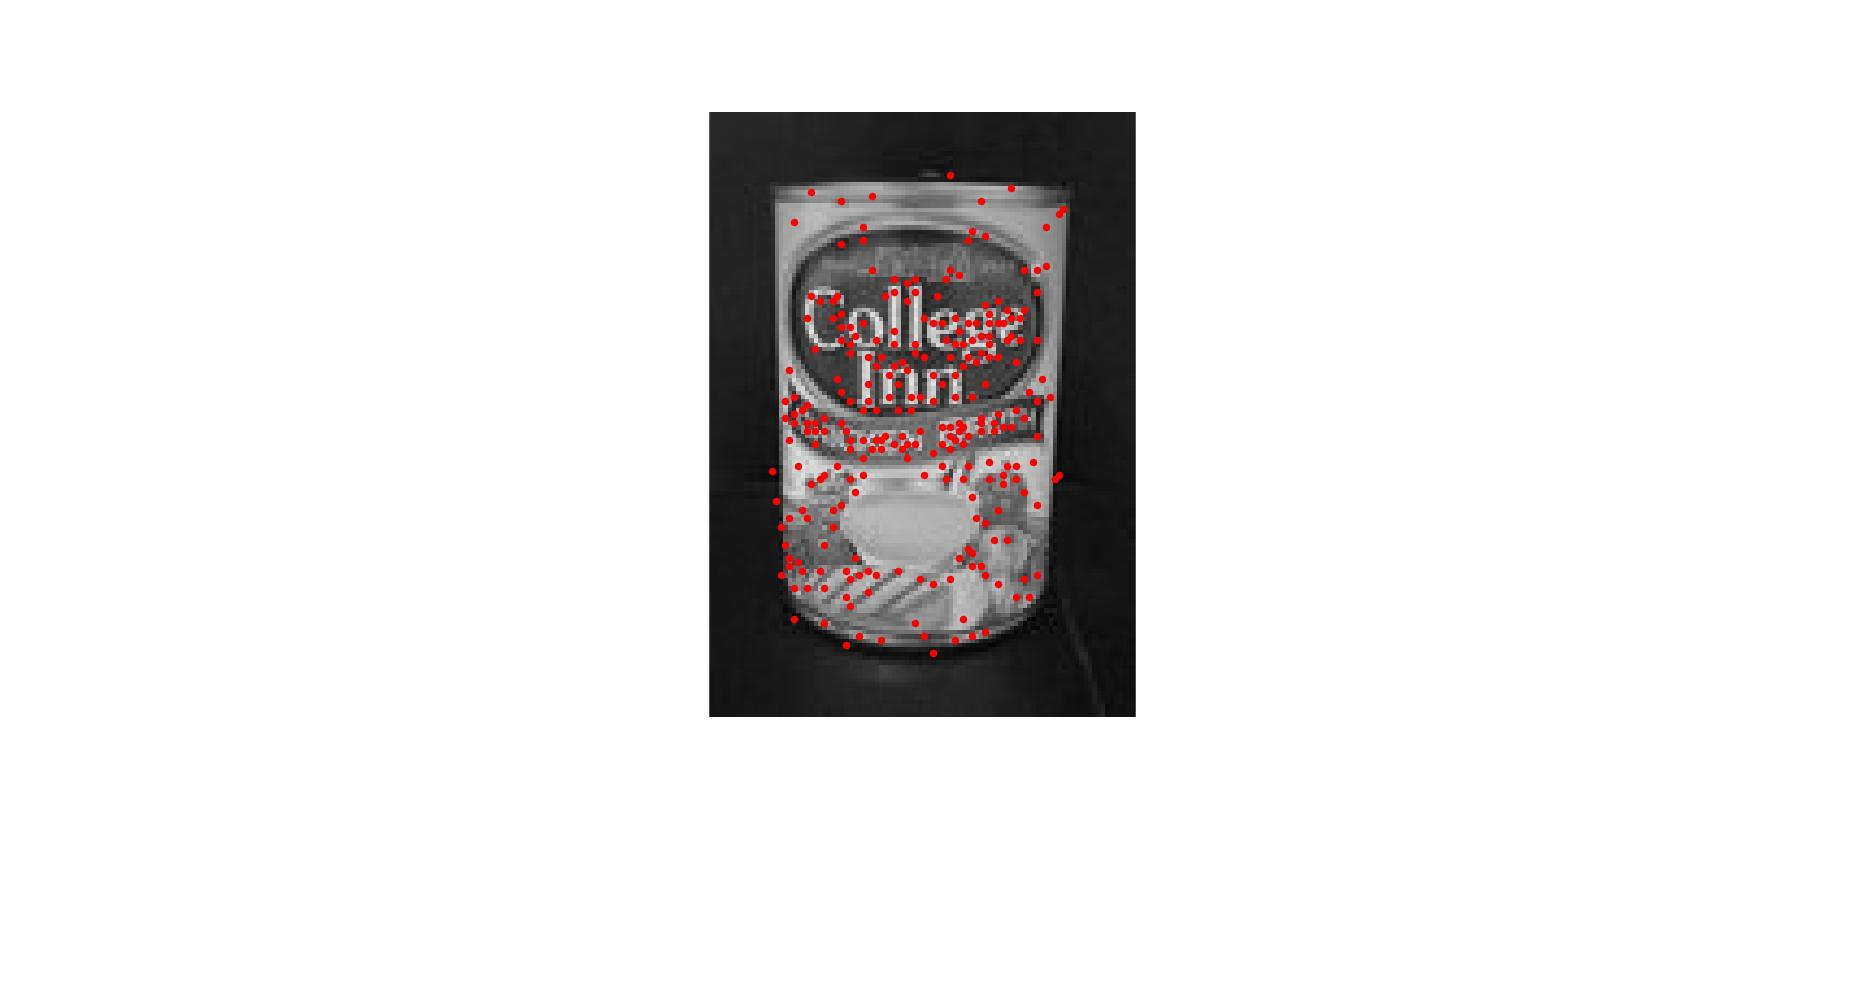
\includegraphics[width=3.0in]{q-1}
    \caption{key-points on \textit{model\_chickenbroth.jpg}}
\end{figure}
\subsection*{2.4}
The following are different results from the matching
\begin{figure}[H]
    \centering
    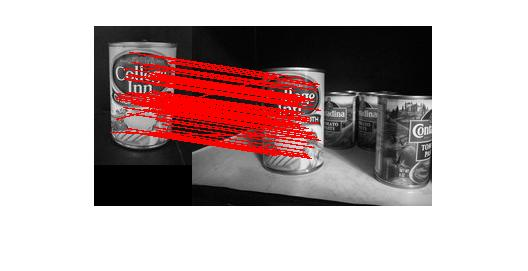
\includegraphics[width=3.0in]{q2-4-1-1}
    \caption{matches between \textit{model\_chickenbroth.jpg} and \textit{chickenbroth\_01.jpg}}
\end{figure}
There are nearly perfect matches, showing that my BRIEF algorithm is correct
\begin{figure}[H]
    \centering
    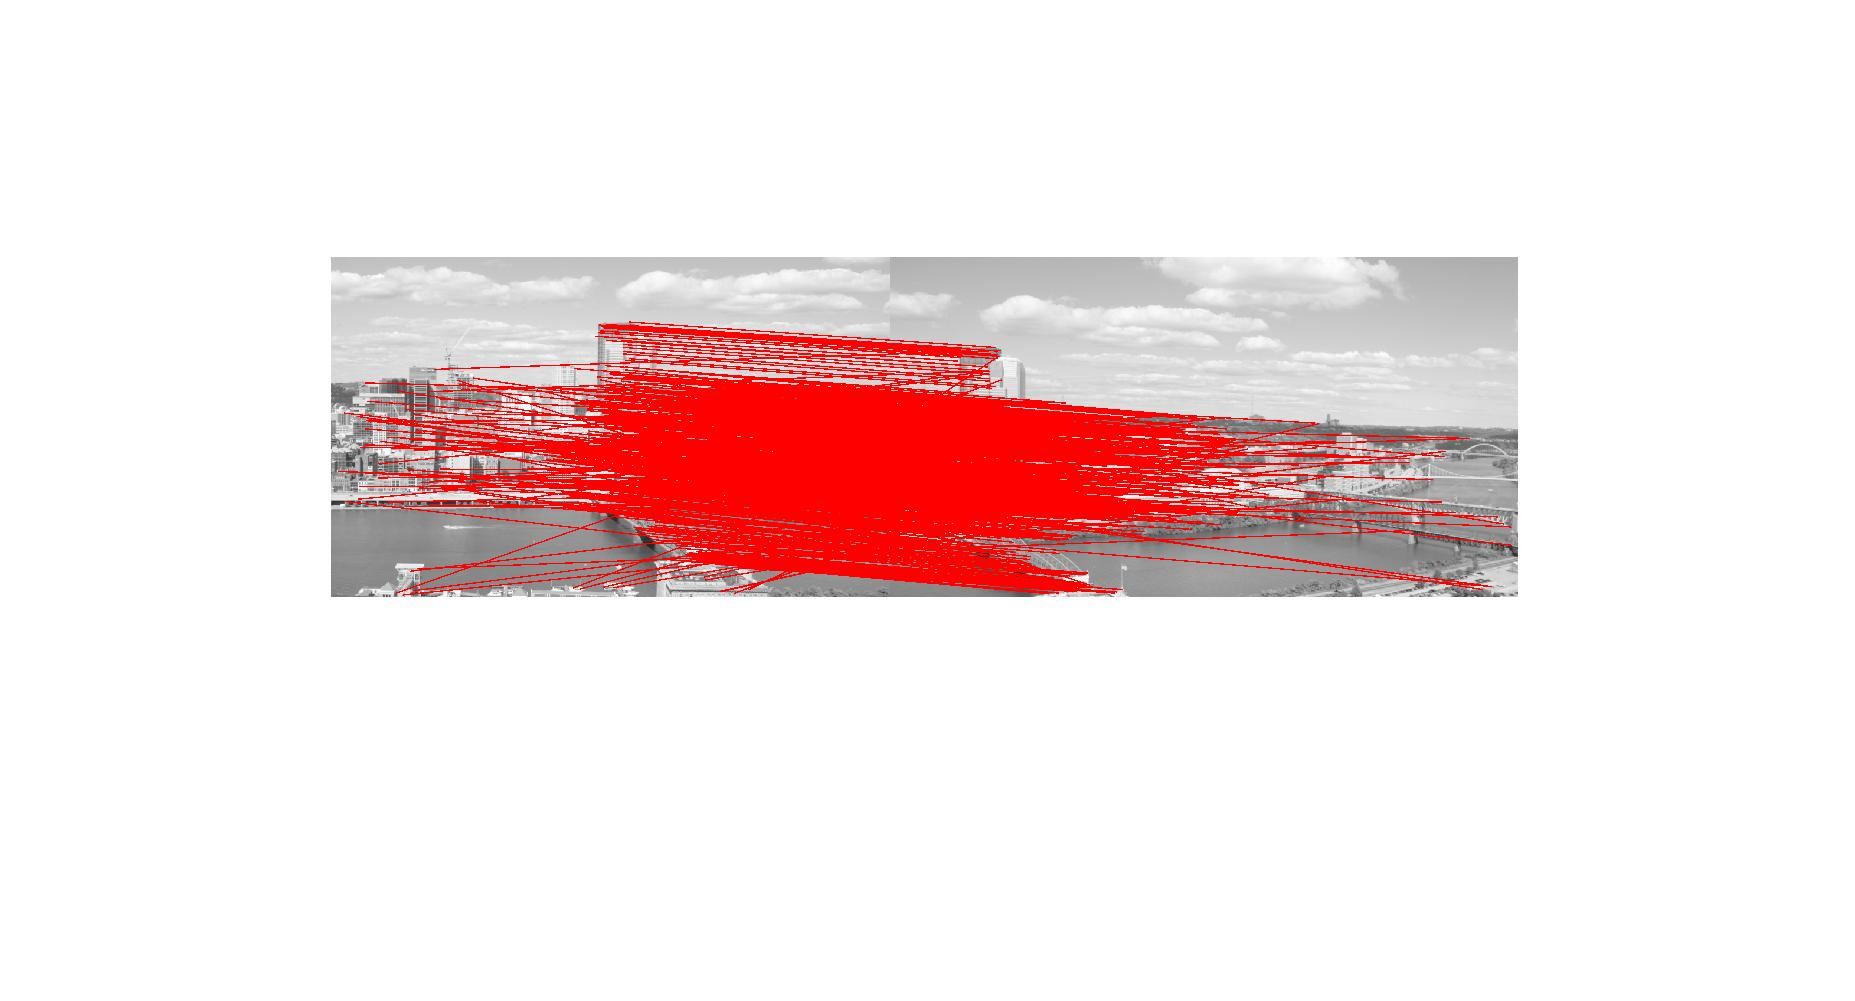
\includegraphics[width=3.0in]{q2-4-1-2}
    \caption{matches between \textit{incline\_l.jpg} and \textit{incline\_r.jpg}}
\end{figure}
Again, we see nearly perfect matches with some error. The repeated part in the image has nearly perfect matches.
\begin{figure}[H]
    \centering
    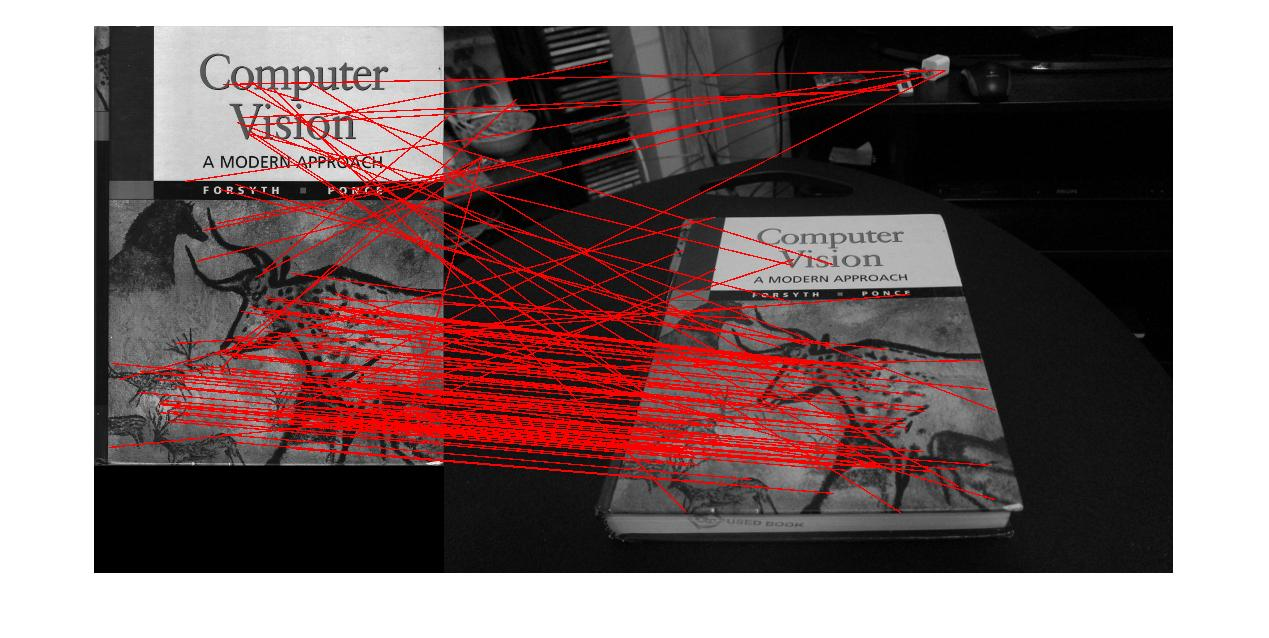
\includegraphics[width=3.0in]{q2-4-1-3}
    \caption{matches between \textit{pf\_scan\_scaled.jpg} and \textit{pf\_desk.jpg}}
\end{figure}
Here we see the effect of skew on BRIEF, the further away the object is from the camera vertically(skew), the worse the matches(the matches are focused on the front). This might because of the features in the front has more pixels are create similar descriptors where the features further in the back are more packed together.
\begin{figure}[H]
    \centering
    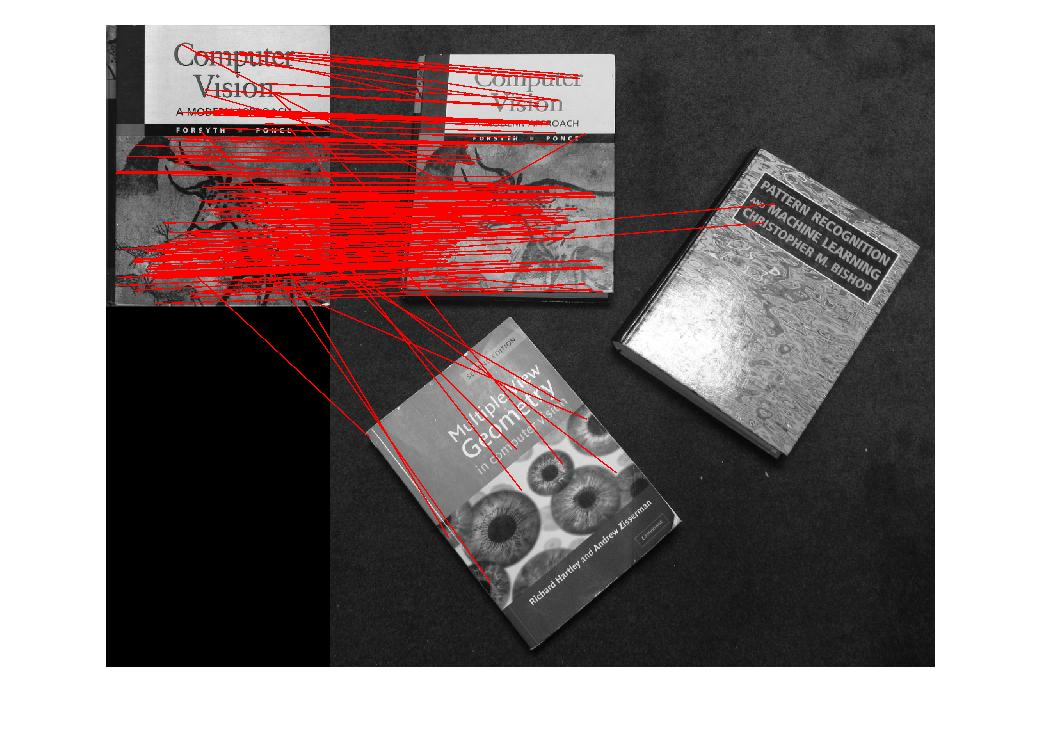
\includegraphics[width=3.0in]{q2-4-1-floor}
    \caption{matches between \textit{pf\_scan\_scaled.jpg} and \textit{pf\_floor.jpg}}
\end{figure}
We have nearly perfect matches, this is because the image is not skew or rotated and have a similar scale.
\begin{figure}[H]
    \centering
    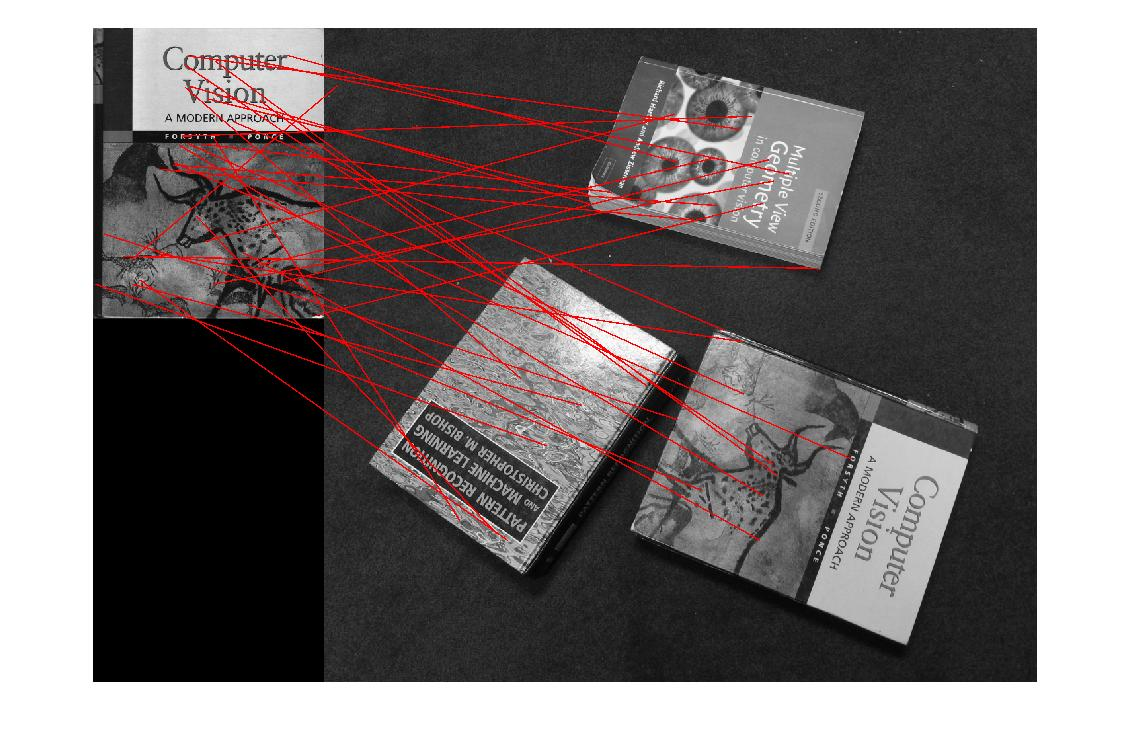
\includegraphics[width=3.0in]{q2-4-1-floor_rot}
    \caption{matches between \textit{pf\_scan\_scaled.jpg} and \textit{pf\_floor\_rot.jpg}}
\end{figure}
The failure to find any matches show that BRIEF doesn't work well with rotation without changes. More of the cause is explored in \textbf{2.5}.
\begin{figure}[H]
    \centering
    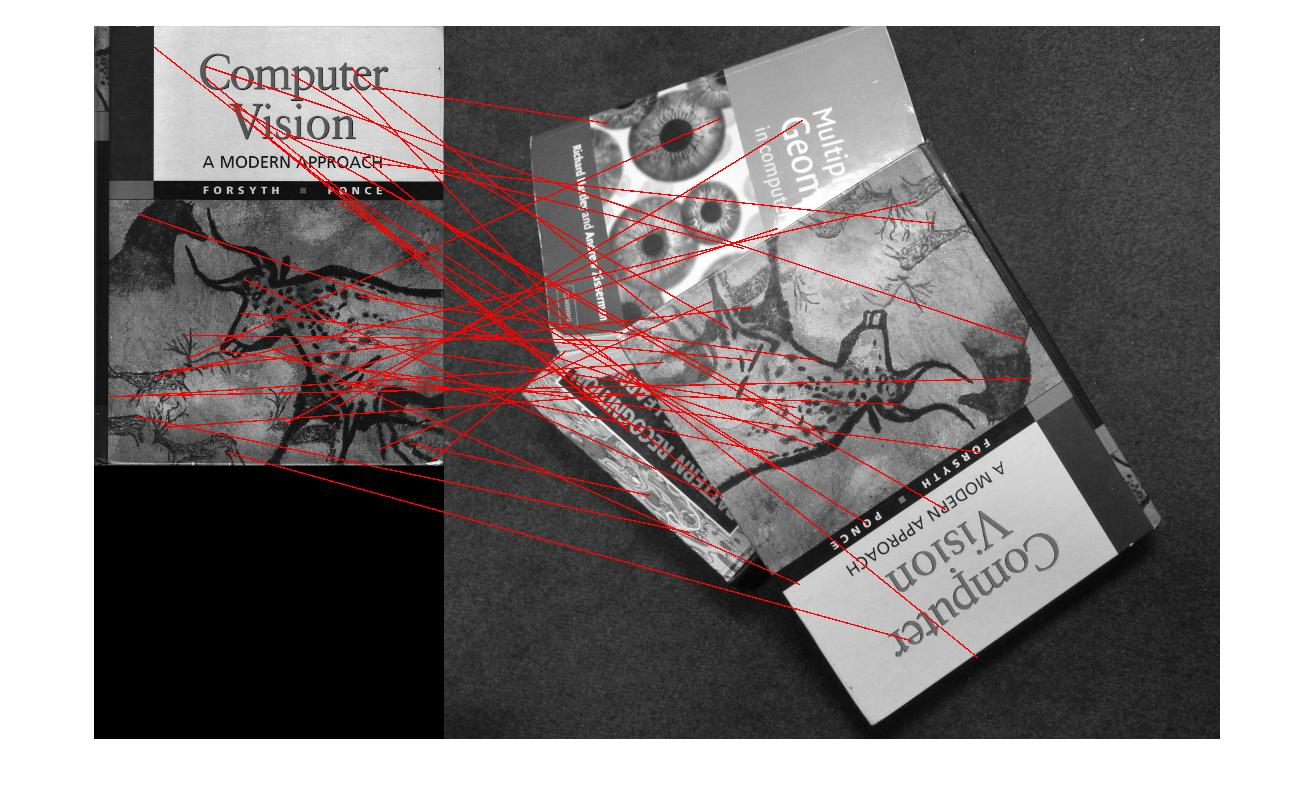
\includegraphics[width=3.0in]{q2-4-1-pile}
    \caption{matches between \textit{pf\_scan\_scaled.jpg} and \textit{pf\_pile.jpg}}
\end{figure}
Again, the match image is rotated around causing bad matches
\begin{figure}[H]
    \centering
    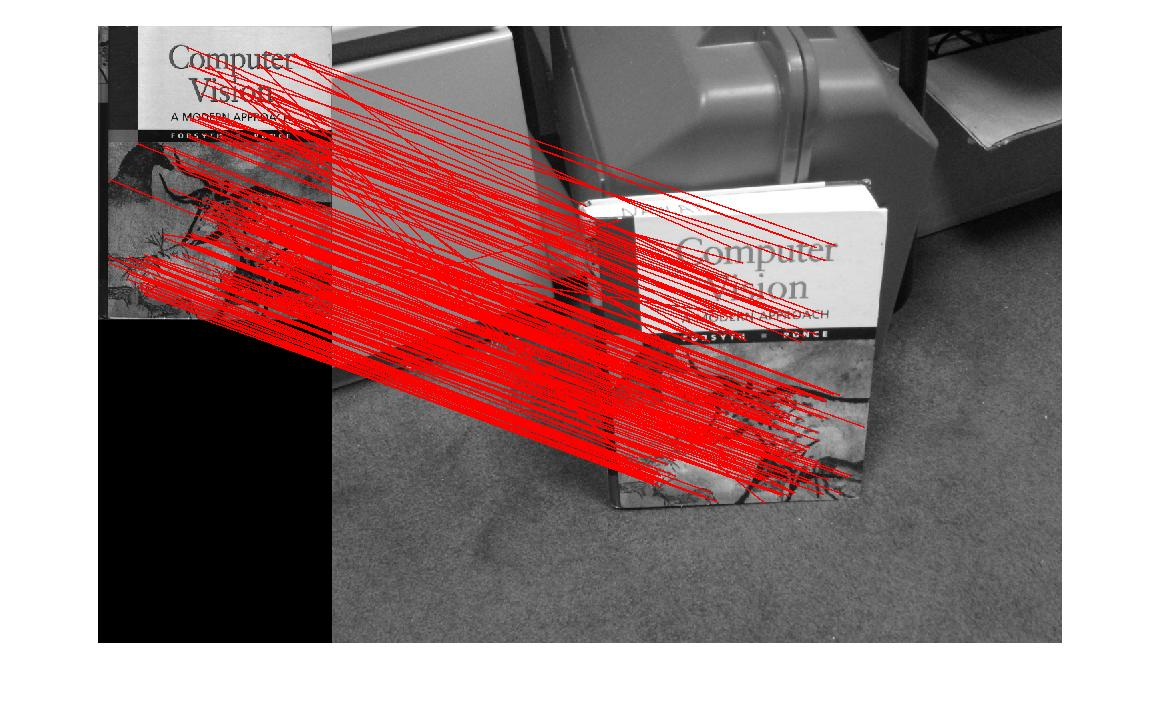
\includegraphics[width=3.0in]{q2-4-1-stand}
    \caption{matches between \textit{pf\_scan\_scaled.jpg} and \textit{pf\_stand.jpg}}
\end{figure}
While the book is stand up in the picture, the angle of the camera created an image where the book is nearly parallel to the model image, giving us good results.

\subsection*{2.5}
\begin{figure}[H]
    \centering
    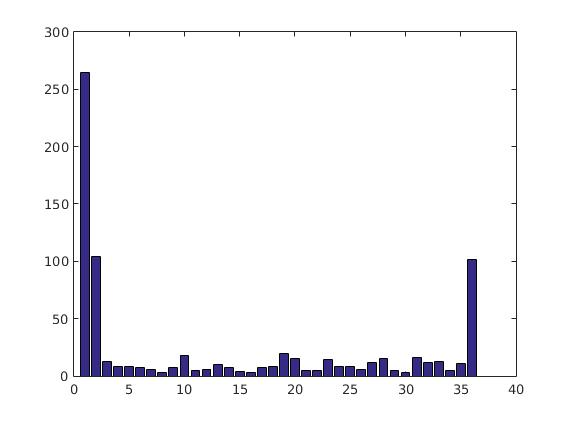
\includegraphics[width=3.0in]{q2_5}
    \caption{Q2.5 question}
\end{figure}
The graph shows the number of matches as the rotation increase from 0 degrees to 350 degrees. Note that there was maximum matches at 0 degrees, and above normal for 10 degrees and 350 degrees. This shows that BRIEF by default would work only when the image and the model's rotation difference is less than 10 degrees.I believe the descriptor does not work correctly when the image is rotated because as patches rotates and the same test pattern will now test for different pixels.
\subsection*{4(a)}
First the equation could be represented by:
\begin{equation*}
\begin{pmatrix}
x_2\\
y_2\\
z_2\\
\end{pmatrix} =
\begin{pmatrix}
H_{11} & H_{12} & H_{13} \\
H_{21} & H_{22} & H_{23} \\
H_{31} & H_{32} & H_{33} \\
\end{pmatrix}
\begin{pmatrix}
x_1\\
y_1\\
z_1\\
\end{pmatrix}
\end{equation*}
The equation can be written in inhomogeneous coordinates:
\begin{equation*}
\begin{aligned}
x'_2 &= \frac{H_{11}x_1 + H_{12}y_1 + H_{13}z_1}{H_{31}x_1 + H_{32}y_1 + H_{33}z_1}\\
y'_2 &= \frac{H_{21}x_1 + H_{22}y_1 + H_{23}z_1}{H_{31}x_1 + H_{32}y_1 + H_{33}z_1}
\end{aligned}
\end{equation*}
because we are working on homography, we can assume $z_1 = 1$ and we then linearize the previous equation to:
\begin{equation*}
\begin{aligned}
x'_2(H_{31}x_1 + H_{32}y_1 + H_{33}) =& H_{11}x_1 + H_{12}y_1 + H_{13}\\
y'_2(H_{31}x_1 + H_{32}y_1 + H_{33}) =& H_{21}x_1 + H_{22}y_1 + H_{23}
\end{aligned}
\end{equation*}
We can break down the first equation into:
\begin{equation*}
\begin{aligned}
H_{31}x_1x'_2 + H_{32}y_1x'_2 + H_{33}x'_2 =& H_{11}x_1 + H_{12}y_1 + H_{13}\\
-H_{11}x_1 - H_{12}y_1 - H_{13} + H_{31}x_1x'_2 + H_{32}y_1x'_2 + H_{33}x'_2 =& 0
\end{aligned}
\end{equation*}
The second equation could also be break into:
\begin{equation*}
\begin{aligned}
H_{31}x_1y'_2 + H_{32}y_1y'_2 + H_{33}y'_2 =& H_{21}x_1 + H_{22}y_1 + H_{23}\\
-H_{21}x_1 - H_{22}y_1 - H_{23} + H_{31}x_1y'_2 + H_{32}y_1y'_2 + H_{33}y'_2 =& 0
\end{aligned}
\end{equation*}
Those two equations could then be written in a matrix form
\begin{equation}
\begin{pmatrix}
	-x_1 & -y_1 & -1 & 0 & 0 & 0 & x_1 x'_2 & y_1 x'_2 & x'_2 \\
	0 & 0 & 0 &-x_1 & -y_1 & -1 & x_1 y'_2 & y_1 y'_2 & y'_2 \\
\end{pmatrix}
\begin{pmatrix}
H_{11}\\
H_{12}\\
H_{13}\\
H_{21}\\
H_{22}\\
H_{23}\\
H_{31}\\
H_{32}\\
H_{33}\\
\end{pmatrix}
= 0
\end{equation}
\subsection*{4(b)}
There are 9 elements in \textbf{h}.
\subsection*{4(c)}
\textbf{H} has 8 degrees of freedom. Because each pair of points create two equations in the matrix.To solve \textbf{H}, we need 4 point correspondences.
\subsection*{4(d)}
To estimate \textbf{h}, we are trying to minimize this equation:
\begin{equation*}
min ||Uh||^2
\end{equation*} 
Where U is the first matrix in equation 1. you first build the matrix $U$ using at least 4 point correspondence. The more points you use, the better your result would be. Then you square the length of the matrix, which is also equal to the matrix's transpose times with itself. After that, I used SVD on the matrix given by $U^TU$ which gives $U\Sigma V^T$. Then I find the least eigenvalue, given by the lowest diagonal element in the diagonal matrix given by SVD and find the corresponding column in $V$. That corresponding column in $V$ is the best estimate of $h$ of $H$.
\subsection*{4.2}
We know both points are pointing at the same location, therefore this equation will hold true:
\begin{equation*}
K_1[I 0]P = K_2[R 0]P'
\end{equation*}
By rearranging the equation, we could create an equation that fits $p \equiv H q$.
\begin{equation*}
\begin{aligned}
K_1[I|0]P =& K_2[R|0]P'\\
K_1[I|0]P =& K_2R[I|0]P'\\
K_1P =& K_2RP'\\
P =& K_2RK'_1P'
\end{aligned}
\end{equation*}
Note that $[I|0]$ could become $I$ as we drop the 4th column, because there are no translation in both the matrices. This also allow us to drop the 4th row on both $P$. 
where $K'_1$ is the inverse of $K_1$. The portion $K_2RK'_1$ is a 3x3 matrix, which is the same as a $H$ matrix. This shows there exist at least a $H$ matrix for two cameras that are rotated.

\subsection*{7.2}
Following is the result of the algorithm at question 7.2:
\begin{figure}[h]
    \centering
    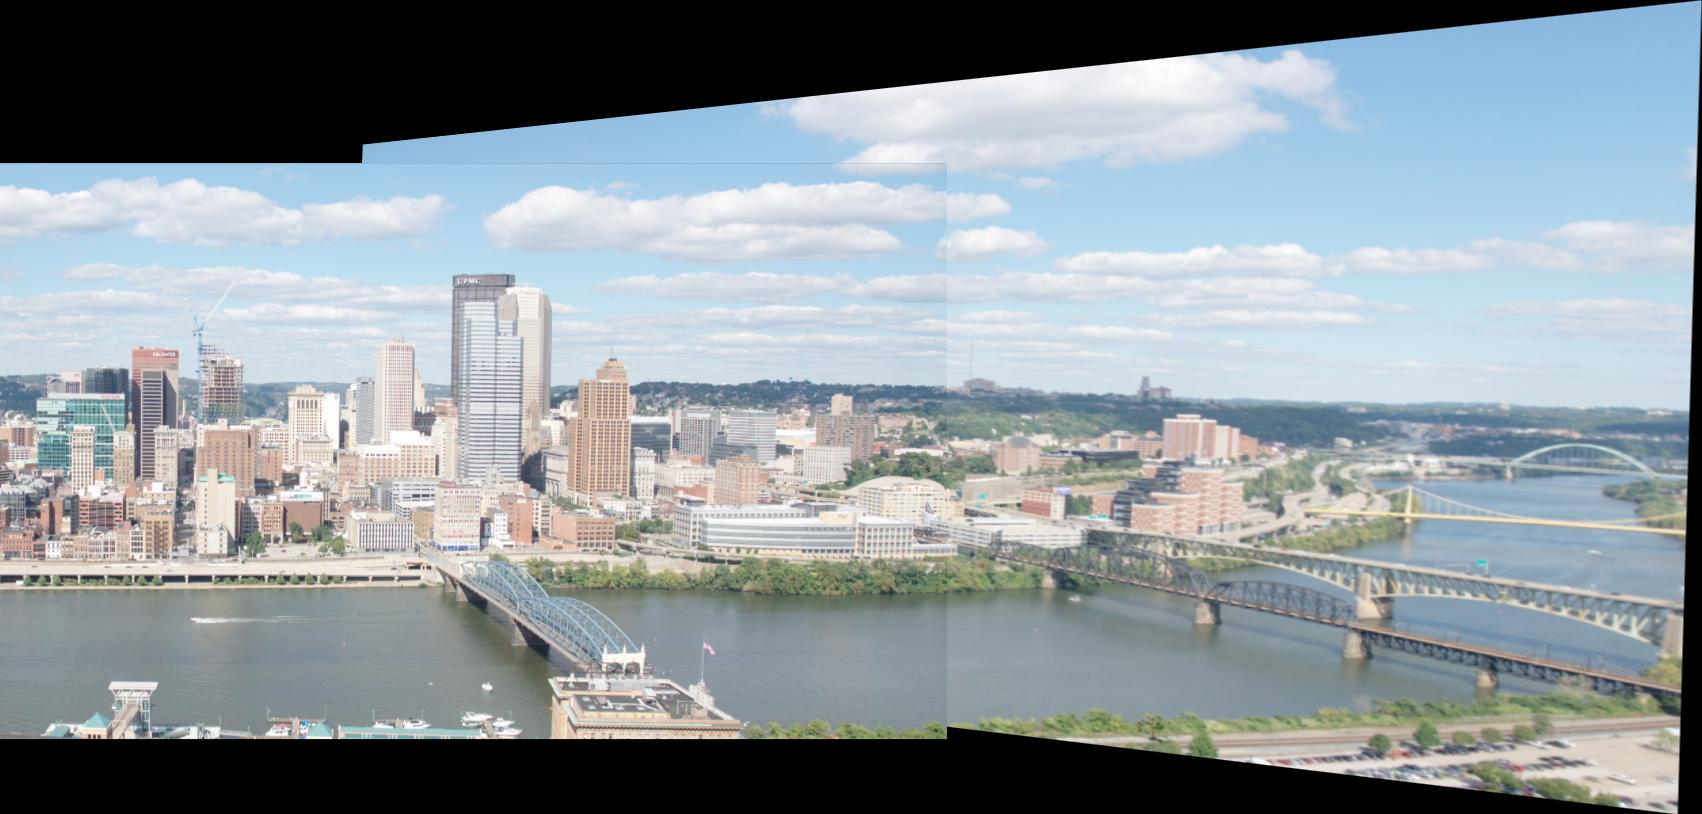
\includegraphics[width=3.0in]{./results/q7_2_pan}
    \caption{Q7.2 The final panaromic image}
\end{figure}
\subsection*{8}
I also attempted the extra credit
\begin{figure}[h]
    \centering
    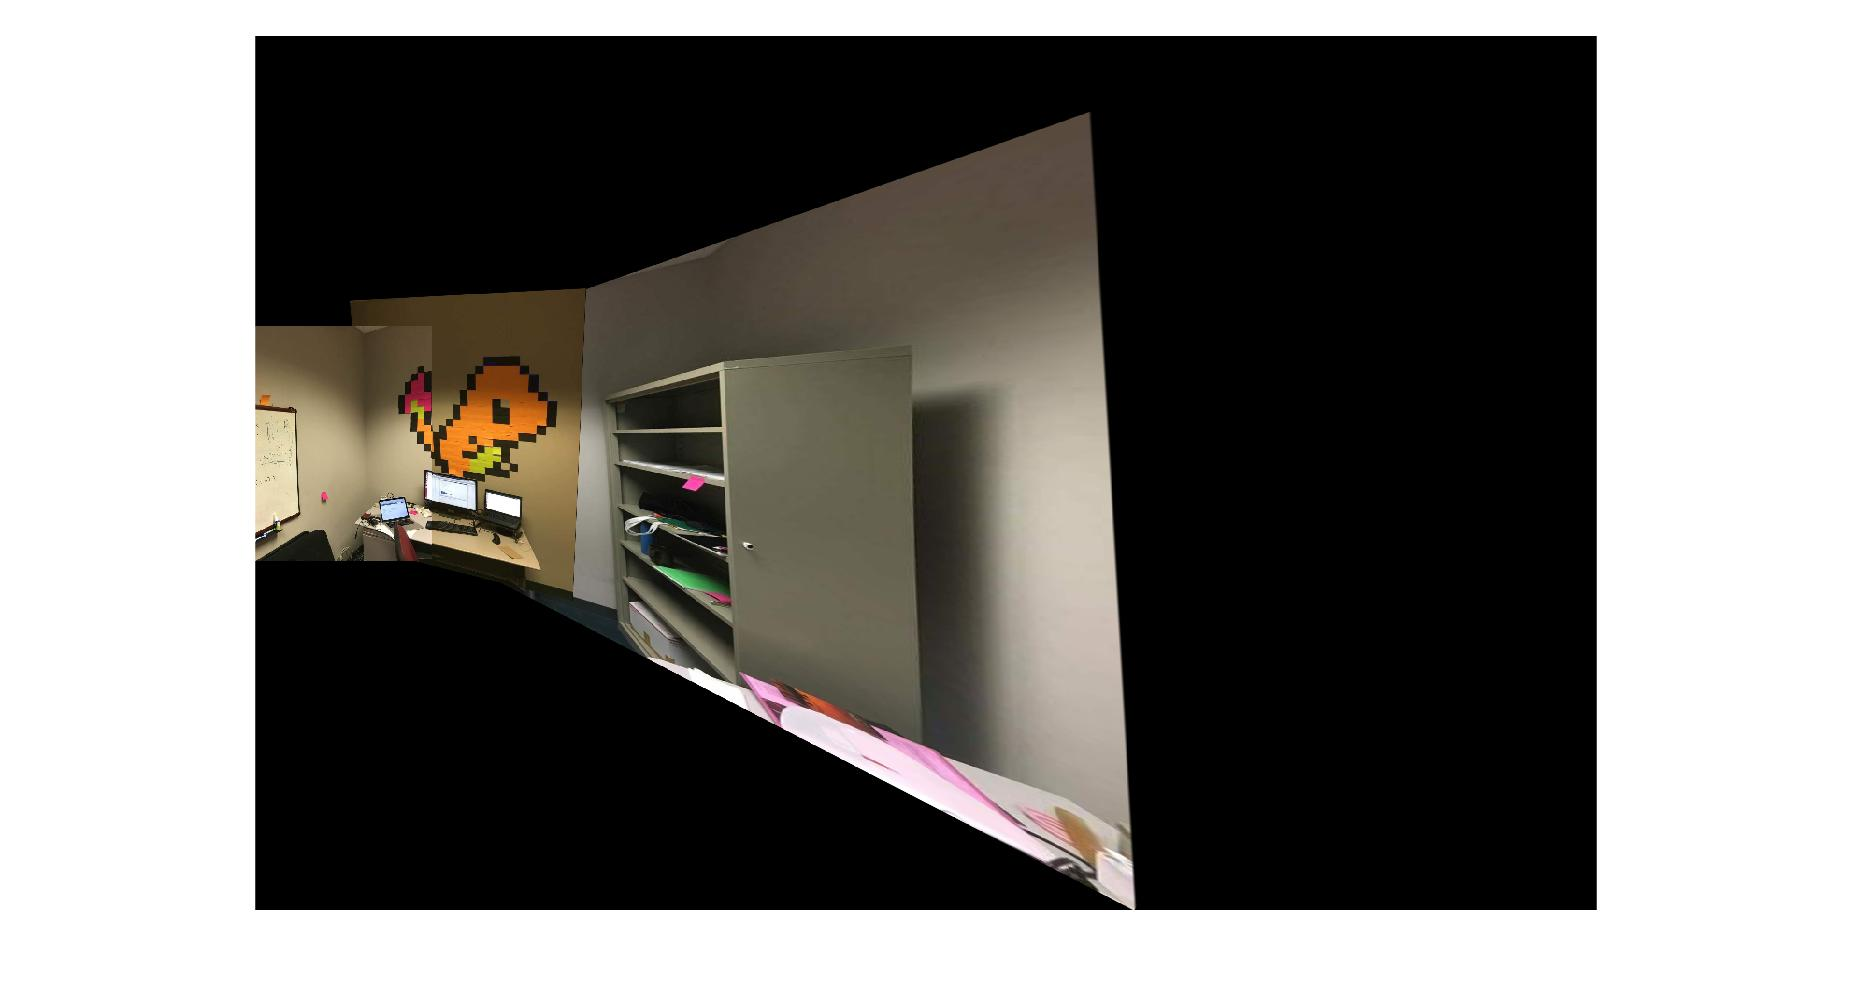
\includegraphics[width=3.0in]{./results/ec8_pan}
    \caption{The combination of all 3 images}
\end{figure}

\end{document}